\section{\uppercase{Features}}
\label{sec:features}
As mentioned in Section~\ref{sec:introduction}, the proposed system is
trained over primarily three types of features. For each file $f$, we
show below how these features are calculated.
\begin{enumerate}
\item \textbf{Folder features.} Typically, the files in a file system
  are organized into folders and sub-folders, with the intent of
  placing together files that are expected to be used together or are
  related to the same task. Our aim is to capture the folder that a
  file belongs to, and to capture the proximity between folders with
  respect to the file system hierarchy without having to explicitly
  define a folder to folder proximity metric. Let's say that the
  folders in the file system are represented by $\mathbf{\mathcal{F}}$
  where $\mathcal{F}(i)$ represents the $i^{th}$ folder. The folder
  features of a file $f$ are represented as the vector
  $\mathbf{X_{f,\mathcal{F}}}$ where the cardinality of
  $\mathbf{X_{f,\mathcal{F}}}$ is the number of folders in the file
  system, i.e., $\mid \mathcal{F} \mid$. The $i^{th}$ element of
  $\mathbf{X_{f,\mathcal{F}}}$, i.e., $X_{f,\mathcal{F}}(i)$ is 1 if
  $\mathcal{F}(i)$ lies in the path of file $f$. For example, if $f$
  is `$\backslash folder1 \backslash folder2 \backslash filename$'
  then $\mathbf{X_{f,\mathcal{F}}}$ would be [1, 1, 0, 0, 0, ...]
  where the first index of $\mathbf{X_{f,\mathcal{F}}}$ corresponds to
  the folder `$\backslash folder1 \backslash$' and the second index
  corresponds to the folder `$\backslash folder1 \backslash folder2
  \backslash$'.
%1 at indices corresponding to the folders `$folder1$', and `$folder1 \backslash folder2$', and 0 for other indices. 
\item \textbf{Token features.}  In addition to folder organization,
  the nomenclature of files and folders also provides useful insights
  into file content and categorization. In order to capture this, we
  tokenize the file path including the file name, and construct a
  vocabulary based on the popular tokens (keywords). Each file is then
  represented as a bag of words based on the constructed vocabulary,
  and based on the tokens present in its path name. Specifically, if
  $\mathcal{T}$ is the set of tokens in the constructed vocabulary,
  then the token features of file $f$ are represented as the vector
  $\mathbf{X_{f,\mathcal{T}}}$ where the cardinality of
  $\mathbf{X_{f,\mathcal{T}}}$ is equal to $\mid \mathcal{T} \mid$.
  The $i^{th}$ element of $\mathbf{X_{f,\mathcal{T}}}$, i.e.,
  $X_{f,\mathcal{T}}(i)$ is equal to the number of times the $i^{th}$
  token is present in the path of $f$.  Section~\ref{sec:tokenization}
  details the tokenization strategy that addresses concatenation of
  entities, something quite common in enterprise metadata.

%Details about the procedure used for tokenization of file path are given in Section~\ref{sec:tokenization}.

\item \textbf{Extension features.}  In order to understand users'
  affinities towards certain types of files, we record the file
  extension as a categorical feature. To utilize this in our models,
  we construct a vocabulary based on popular file extensions in the
  share, $\mathcal{E}$. We then represent the extension of a file $f$
  by a binary vector $\mathbf{X_{f, \mathcal{E}}}$ where the $i^{th}$
  value of $\mathbf{X_{f, \mathcal{E}}}$, i.e., $X_{f,
    \mathcal{E}}(i)$ is 1 if $f$ has the $i^{th}$ extension, and is 0
  otherwise. Cardinality of $\mathbf{X_{f, \mathcal{E}}}$ is equal to
  $\mid \mathcal{E} \mid$.
\end{enumerate}
For a file $f$, the metadata feature vector $\mathbf{X_f}$ is obtained
by concatenating the above three types of features. Specifically, for
file $f$, the metadata feature vector is obtained as
\begin{equation}
\label{eq:featurevector}
\mathbf{X_f} = \lbrack  \mathbf{X_{f,\mathcal{F}}} \; \; \; , \;  \;  \;  \mathbf{X_{f,\mathcal{T}}} \; \; \; , \;  \;  \;  \mathbf{X_{f, \mathcal{E}}}  \rbrack. 
\end{equation}
% We can just roll into the next section

\section{\uppercase{Modeling}}
\label{sec:models}
In order to model users' file access patterns, we define a training
period to train the models, and a testing period to evaluate. We
follow a personalized modeling approach where we train one model for
each user.
%
%
For evaluation, we select 30
users based on the number of file activities of all users in a
share.
%
%
Details on the selection of evaluation users are provided in
Section~\ref{sec:selectusers}. All files that were operated on during
the training period by at least one user in the share are the training
instances. For user $u$, the training label of a file is 1 if $u$
accessed the file during training period, 0 otherwise.  Testing
instances are the files that are operated upon in testing period,
after removing the files that were observed in the training
period. This ensures that the testing files are new relative to the
training files. The testing labels are determined in the same fashion
as for training.  Note that we only focus on training and testing
over file read events. The total set of training instances is
the same across all users, but the labels can differ. The same holds
for testing.  The overall approach is described in
Figure~\ref{fig:overallApproach}(a).
\begin{figure}[h!]
\begin{center}
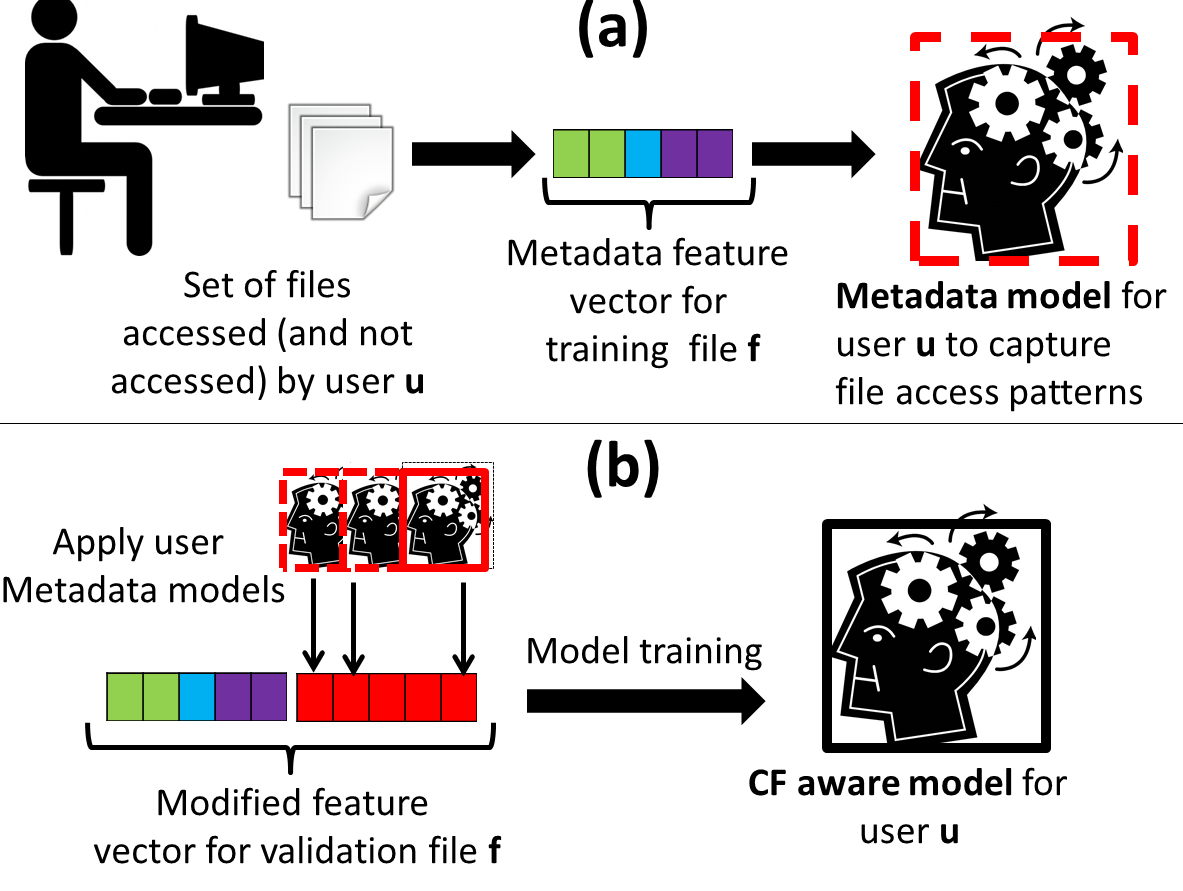
\includegraphics[width=0.95\linewidth]{FileAccess/figs/overall_framework}
\caption{Overall approach of the proposed system. a) shows the training of user models based on only metadata features (metadata models). The files accessed by users are represented in terms of their metadata features, followed by training of the metadata model. b) shows how individual metadata user models are applied on validation files to train collaborative filtering (CF) aware models (Section~\ref{sec:collabfiltering}). } 
\label{fig:overallApproach}
\end{center}
\end{figure}
We approach the modeling of file access patterns and its evaluation as
a classification problem and utilize the features detailed in
Section~\ref{sec:features}.
%%
%% sandeep: Why are experiments described in this section
%%

\subsection{Collaborative filtering aware modeling}
\label{sec:collabfiltering}
As discussed in Section~\ref{sec:data}, file accesses typically
demonstrate a high degree of collaboration among users as evidenced by
the triangle count. The features defined in Section~\ref{sec:features}
only capture metadata attributes of files. The models trained on these
features can be improved by utilizing the predictions from models of
other users in the same share. With this motivation, we describe how the
system augments the personalized user models with additional
information to achieve collaborative filtering.

Figure \ref{fig:overallApproach}(b) shows the modified approach to
make the trained models aware of the collaboration among users. We
obtain validation instances from the training instances. There are
several ways to do so. We experimented with sampling validation
instances from training instances for different sampling rates. The
best performance, however, was observed when the validation set was
kept the same as the training set.
%For explanation purpose using Figure~\ref{fig:overallApproach}(b),
On the other hand, the testing set, as required, is completely
independent of the training or validation set.

%We will treat training and validation instances separately. The
%testing set is defined based on the testing period and is only used
%for evaluation. Nothing from the testing period is utilized to
%construct features, or to train the models.

Let $U$ represent the set of users in a share. The models labeled with
``Metadata models" in Figure \ref{fig:overallApproach} represent the
$\mid U \mid$ personalized classification models based on the metadata
features. Each of the metadata models is trained over the training
instances, and applied on the validation instances. For a file $f$
among the validation instances, the predicted labels from metadata
models are concatenated to form $\mathbf{P_{f,U}}$ where the $j^{th}$
value i.e., $P_{f,U}(j)$ is equal to the predicted label of the
validation instance $f$ by the metadata model for the $j^{th}$ user in
the share. These predicted labels are concatenated with the metadata
feature vector of the validation instances to form the feature vector
for a second layer of models. Specifically,
\begin{equation}
\label{eq:featurevectorCollab}
\mathbf{X^{c}_f} = \lbrack  \mathbf{X_f}  \; \; \; , \;  \;  \;  \mathbf{P_{f,U}}     \rbrack, 
\end{equation}
and the second layer of models are binary classification models
trained with $\mathbf{X^{c}_f}$ as the feature vector for each
validation file $f$. These collaborative filtering aware models are
represented as ``CF aware" models in
Figure~\ref{fig:overallApproach}(b).


During the testing phase, the predicted label for a given user $u$ on
a test file $f$ is obtained as follows. First the metadata models of
all the users in $U$ are applied on $f$ to obtain their predicted labels.
These labels are then concatenated with the metadata features of $f$ as shown in Eq.~\ref{eq:featurevectorCollab}.  Finally, the
predicted label for a user is obtained by applying her CF aware model on
the concatenated feature vector of $f$.

%% In the testing phase, first the metadata models are applied to obtain
%% $\mathbf{P_{f,U}}$ for each testing file $f$. The predicted labels of
%% these models are then concatenated with the metadata features of the
%% files as shown in Eq.~\ref{eq:featurevectorCollab}. The CF aware model
%% for user $u$ is then applied on the constructed feature vectors to get
%% the predicted label for user $u$ and testing file $f$.

Constructing CF aware user models based on the above approach has two
key advantages. First, CF aware models can leverage collaboration by
factoring the predicted labels of other users' metadata models. It
should be noted that this approach does not require explicitly
defining a similarity metric between users or their access patterns,
and yet enables the model to improve its predictive performance.  For
example, if the users $u_1$ and $u_2$ have similar behavior, it can be
expected that the validation files for which the metadata model of
$u_1$ predicts a positive label, are also likely to be accessed by
$u_2$.  Now consider a third user $u_3$ whose behavior is very
different from that of $u_1$ and $u_2$.  Thus, if the metadata model
of $u_3$ predicts a positive label for a validation file $f$, the
likelihood of the user $u_1$ or $u_2$ accessing $f$ would
automatically decrease. The CF model can leverage such learned
knowledge of similar and dissimilar access patterns to improve its
correctness.

The second advantage of our CF aware modeling is that it does not
suffer from the cold start problem that the traditional collaborative
filtering systems suffer from. To make recommendations to the user
$u$, these systems first identify other users who share similar
preferences with $u$, and then propose items which were favored by the
other users but not seen by $u$.  Such systems fail to make
recommendation for a completely new item.  Our approach gets around
the cold start problem by utilizing the predicted labels of users in a
share along with the metadata features.  In
Section~{\ref{sec:CFevaluation}}, we show how the CF aware models
improve the classification performance over the metadata models.  With
a higher degree of collaboration, we are expected to observe higher
gains of the CF aware model. Our results strongly corroborate this
observation.
